\documentclass[aspectratio=169,t]{beamer}

\usetheme{Madrid}
\setbeamertemplate{navigation symbols}{}

\usepackage[utf8]{inputenc}
\usepackage[T1]{fontenc}
\usepackage[spanish]{babel}
\shorthandoff{.<>"}
\usepackage{graphicx}
\usepackage{booktabs}
\usepackage{listings}
\usepackage{xcolor}
\usepackage{tikz}
\usetikzlibrary{positioning,arrows.meta}

\definecolor{azulUSM}{RGB}{0,58,122}
\definecolor{rojoDBA}{RGB}{214,39,40}

\lstdefinestyle{pseudo}{
    basicstyle=\ttfamily\scriptsize,
    keywordstyle=\bfseries\color{azulUSM},
    commentstyle=\itshape\color{gray},
    morekeywords={mientras,si,sino,retorna,funcion,fin,agendar,encolar},
    breaklines=true,
    frame=single,
    framerule=0.3pt,
    backgroundcolor=\color{black!4},
    xleftmargin=6pt,
    xrightmargin=6pt,
    showstringspaces=false,
}

\graphicspath{{../../../figures/}}

\title[XG-PON: SLA y DBA]{Simulador XG-PON: IPACT vs GIANT vs QoSDBA}
\subtitle{Cumplimiento de SLA en una red de acceso óptica}
\author[OmneTeam]{David Retuerto \and José Vega \and Matías Perelli}
\institute[UTFSM]{TEL-341 Simulación de Redes\\Universidad Técnica Federico Santa María}
\date{2026}

\begin{document}

\begin{frame}
    \titlepage
\end{frame}

\begin{frame}{Agenda}
    \tableofcontents
\end{frame}

\section{Introducción}

\begin{frame}{Motivación}
    \textbf{Proyecto 2 (Fase 2):} simulamos GPON ITU-T G.984, 32 ONUs,
    comparando un DBA proporcional contra uno con QoS por T-CONT.

    \vspace{0.2cm}
    \textbf{Pivote a esta Fase 3} (reunión con la profesora, 9/6/2026):
    \begin{itemize}
        \item Migrar a \textbf{XG-PON1 (ITU-T G.987)}, el sucesor 10G de GPON
        \item Reducir a \textbf{8 ONUs idénticas} y exigir una meta de SLA
              explícita para VoIP ($\leq$ 2 ms)
        \item Comparar \textbf{IPACT} (polling de EPON, usado a propósito
              como referencia) contra dos algoritmos nativos de PON
              (\textbf{GIANT}, \textbf{QoSDBA})
    \end{itemize}

    \vspace{0.2cm}
    Pregunta que motiva todo el proyecto: \textbf{¿el algoritmo de DBA
    importa para que una llamada de voz cumpla su SLA de latencia?}
\end{frame}

\section{El problema}

\begin{frame}{Por qué hace falta un algoritmo}
    Una PON conecta una central (OLT) con varios usuarios (ONUs) usando un
    solo cable de fibra, repartido por un splitter pasivo.

    \begin{itemize}
        \item Bajada (OLT a ONUs): no hay problema, la señal le llega a todos.
        \item Subida (ONUs a OLT): todas las ONUs comparten el mismo canal,
              solo una puede transmitir a la vez.
    \end{itemize}

    \vspace{0.3cm}
    Si por ese mismo canal compiten cosas muy distintas, como una llamada
    de voz y una descarga pesada, alguien tiene que decidir quién
    transmite y en qué momento. Esa decisión es el corazón de este
    proyecto.
\end{frame}

\section{La red simulada}

\begin{frame}{La red que simulamos: XG-PON1}
    Estándar ITU-T G.987, el sucesor de GPON.

    \begin{center}
    \begin{tikzpicture}[
        box/.style={draw, rounded corners, align=center, minimum height=0.9cm,
                    minimum width=2.4cm, fill=azulUSM!8, font=\footnotesize},
        node distance=0.6cm
    ]
        \node[box] (olt) {OLT};
        \node[box, right=of olt] (split) {Splitter\\1:8};
        \node[box, right=of split] (onu) {8 ONUs};
        \draw[-{Latex[length=2mm]}] (olt) -- node[above, font=\tiny] {20 km de fibra} (split);
        \draw[-{Latex[length=2mm]}] (split) -- (onu);
    \end{tikzpicture}
    \end{center}

    \begin{columns}
        \column{0.5\textwidth}
        \begin{itemize}
            \item Upstream: 2.48832 Gbps
            \item Trama: 125 $\mu$s (8000 por segundo)
        \end{itemize}
        \column{0.5\textwidth}
        \begin{itemize}
            \item 38880 bytes disponibles por trama
            \item Delay de propagación: 100 $\mu$s
        \end{itemize}
    \end{columns}
\end{frame}

\section{T-CONTs}

\begin{frame}{T-CONTs: qué son y cuáles usamos}
    En vez de tener una sola cola para todo el tráfico de una ONU, GPON y
    XG-PON definen \textbf{T-CONTs} (Transmission Containers): una cola
    distinta por tipo de servicio, cada una con su propia prioridad.

    \vspace{0.3cm}
    \begin{table}
        \footnotesize
        \renewcommand{\arraystretch}{1.3}
        \begin{tabular}{lccc}
            \toprule
            T-CONT & Tráfico & Tasa & Paquete \\
            \midrule
            T-CONT1 (VoIP) & CBR (fijo) & 1 Mbps & 160 B \\
            T-CONT2 (Video) & Poisson & 40 Mbps & 1000 B \\
            T-CONT4 (Datos) & Pareto ($\alpha$=1.5) & 200 a 800 Mbps\footnotemark & 1400 B \\
            \bottomrule
        \end{tabular}
    \end{table}
    \footnotetext{Varía según el escenario de carga, ver diseño experimental}
\end{frame}

\section{El SLA}

\begin{frame}{El SLA: qué es y por qué importa}
    Un SLA acá es simple: una cota máxima de latencia. Si un paquete llega
    más tarde que esa cota, se considera que el servicio falló para ese
    paquete.

    \vspace{0.3cm}
    \begin{table}
        \footnotesize
        \renewcommand{\arraystretch}{1.3}
        \begin{tabular}{lcl}
            \toprule
            T-CONT & Cota & Origen \\
            \midrule
            \textbf{T-CONT1 (VoIP)} & \textbf{$\leq$ 2 ms} & \textbf{Pedido explícito de la profesora} \\
            T-CONT2 (Video) & $\leq$ 20 ms & Meta razonable del equipo \\
            T-CONT4 (Datos) & $\leq$ 500 ms & Cota laxa, solo de referencia \\
            \bottomrule
        \end{tabular}
    \end{table}

    \vspace{0.2cm}
    La que de verdad nos interesa demostrar es la de T-CONT1. Las otras
    dos no son normas del estándar, son metas que pusimos nosotros para
    tener algo con qué comparar.
\end{frame}

\section{El problema del DBA}

\begin{frame}{Dynamic Bandwidth Allocation}
    Si cada ONU transmitiera cuando quisiera, habría choques en el canal.
    Alguien tiene que decidir, trama por trama, quién transmite y cuánto.

    \vspace{0.3cm}
    Esa decisión se llama \textbf{DBA} (Dynamic Bandwidth Allocation), y
    es la pregunta de investigación real de este proyecto: ¿qué tan bien
    distintos algoritmos de DBA logran cumplir el SLA de voz?
\end{frame}

\begin{frame}{Dos formas de coordinar el canal}
    \begin{columns}[t]
        \column{0.48\textwidth}
        \textbf{Broadcast (SR-DBA)}\\
        \textit{usado por GIANT y QoSDBA}
        \begin{itemize}
            \item \footnotesize La OLT calcula la asignación de las 8 ONUs de una vez
            \item \footnotesize La manda en un solo mensaje (BWmap), cada 125 $\mu$s exactos
        \end{itemize}
        \column{0.48\textwidth}
        \textbf{Polling}\\
        \textit{usado por IPACT}
        \begin{itemize}
            \item \footnotesize La OLT le habla a una ONU a la vez, en ronda
            \item \footnotesize El ciclo completo dura lo que se necesite: entre 8 y 1008 $\mu$s
        \end{itemize}
    \end{columns}
\end{frame}

\begin{frame}{Los 3 algoritmos comparados}
    \begin{table}
        \footnotesize
        \renewcommand{\arraystretch}{1.4}
        \begin{tabular}{lp{5.2cm}l}
            \toprule
            Algoritmo & Mecanismo & Trama / ciclo \\
            \midrule
            IPACT & Sondea ONU por ONU, otorga el mínimo entre la demanda y un máximo fijo & Variable: 8 a 1008 $\mu$s \\
            GIANT & T-CONT1 reservado siempre, T-CONT2 y T-CONT4 con contadores de turno & Fija: 125 $\mu$s \\
            QoSDBA & Prioridad estricta T-CONT1 $>$ T-CONT2 $>$ T-CONT4 & Fija: 125 $\mu$s \\
            \bottomrule
        \end{tabular}
    \end{table}

    \vspace{0.2cm}
    \footnotesize IPACT es de EPON, otro estándar. Lo usamos a propósito
    como punto de comparación, no porque XG-PON lo use de verdad.
\end{frame}

\section{El simulador}

\begin{frame}{Arquitectura del simulador}
    \footnotesize
    \textbf{Python 3 puro}, sin frameworks de simulación (sin SimPy, sin
    OMNeT++): solo \texttt{heapq} de la librería estándar para la cola de
    eventos.

    \vspace{0.2cm}
    \begin{center}
    \begin{tikzpicture}[
        box/.style={draw, rounded corners, align=center, minimum height=0.85cm,
                    minimum width=7cm, fill=azulUSM!8},
        node distance=0.45cm
    ]
        \node[box] (engine) {Motor de eventos (cola ordenada por tiempo)};
        \node[box, below=of engine] (olt) {OLT: corre el algoritmo DBA};
        \node[box, below=of olt] (canal) {Canal óptico: delay de propagación};
        \node[box, below=of canal] (onu) {ONUs: T-CONTs + generadores de tráfico};
        \draw[-{Latex[length=2mm]}] (engine) -- (olt);
        \draw[-{Latex[length=2mm]}] (olt) -- (canal);
        \draw[-{Latex[length=2mm]}] (canal) -- (onu);
    \end{tikzpicture}
    \end{center}
    \footnotesize
    OLT y ONUs se hablan en los dos sentidos a través del canal:
    asignación hacia abajo, datos y reportes hacia arriba. El motor de
    eventos es lo que hace que todo eso pase en el momento correcto.
\end{frame}

\begin{frame}{Estado del sistema y entidades}
    \footnotesize
    \textbf{Entidades y atributos:}
    \begin{itemize}
        \item \textbf{OLT}: reportes recibidos por ONU, número de trama actual
        \item \textbf{ONU}: un \texttt{TCont} por tipo (1, 2, 4)
        \item \textbf{TCont}: buffer FIFO, bytes encolados, contadores de
              paquetes/bytes generados y descartados
        \item \textbf{Paquete}: ONU de origen, tipo de T-CONT, tamaño,
              instante de creación
        \item \textit{Solo en GIANT}: contadores de turno SImax/SImin por ONU.
              \textit{Solo en IPACT}: índice de la ONU que se está sondeando
    \end{itemize}

    \vspace{0.2cm}
    \textbf{Estado del sistema} en el instante $t$: ocupación de cada
    buffer T-CONT de cada ONU, último reporte (DBRu) conocido por la OLT
    de cada ONU, y los contadores de turno/posición de polling vigentes.
    Ese estado es lo único que el DBA necesita para decidir el siguiente
    BWmap o GATE.
\end{frame}

\begin{frame}{Eventos futuros (FEL) y condición de término}
    \footnotesize
    \begin{table}
        \footnotesize
        \renewcommand{\arraystretch}{1.2}
        \begin{tabular}{ll}
            \toprule
            Evento & Dispara \\
            \midrule
            \texttt{ONU\_GENERATE\_TRAFFIC} & encola paquete, se reagenda a sí mismo \\
            \texttt{OLT\_GENERATE\_BWMAP} & DBA broadcast (GIANT/QoSDBA), cada 125 $\mu$s \\
            \texttt{ONU\_RECEIVE\_BWMAP} & ONU transmite + envía DBRu \\
            \texttt{OLT\_SEND\_GATE} / \texttt{POLL\_NEXT} & DBA polling (IPACT), por ONU \\
            \texttt{ONU\_RECEIVE\_GATE} & ONU transmite + envía DBRu (IPACT) \\
            \texttt{OLT\_RECEIVE\_DATA} & mide latencia, registra entrega \\
            \texttt{OLT\_RECEIVE\_REPORT} & actualiza el reporte de esa ONU \\
            \bottomrule
        \end{tabular}
    \end{table}

    \textbf{Condición de término:} tiempo fijo de simulación
    $[0, T]$ con $T=10$ s, descartando el primer segundo (\textit{warmup},
    8000 tramas) para evitar medir el transitorio de buffers vacíos. Cada
    escenario se corre \textbf{10 veces} con semillas distintas
    (6767-6776) para poder calcular intervalos de confianza.
\end{frame}

\begin{frame}{El loop del simulador, paso a paso}
    \begin{center}
        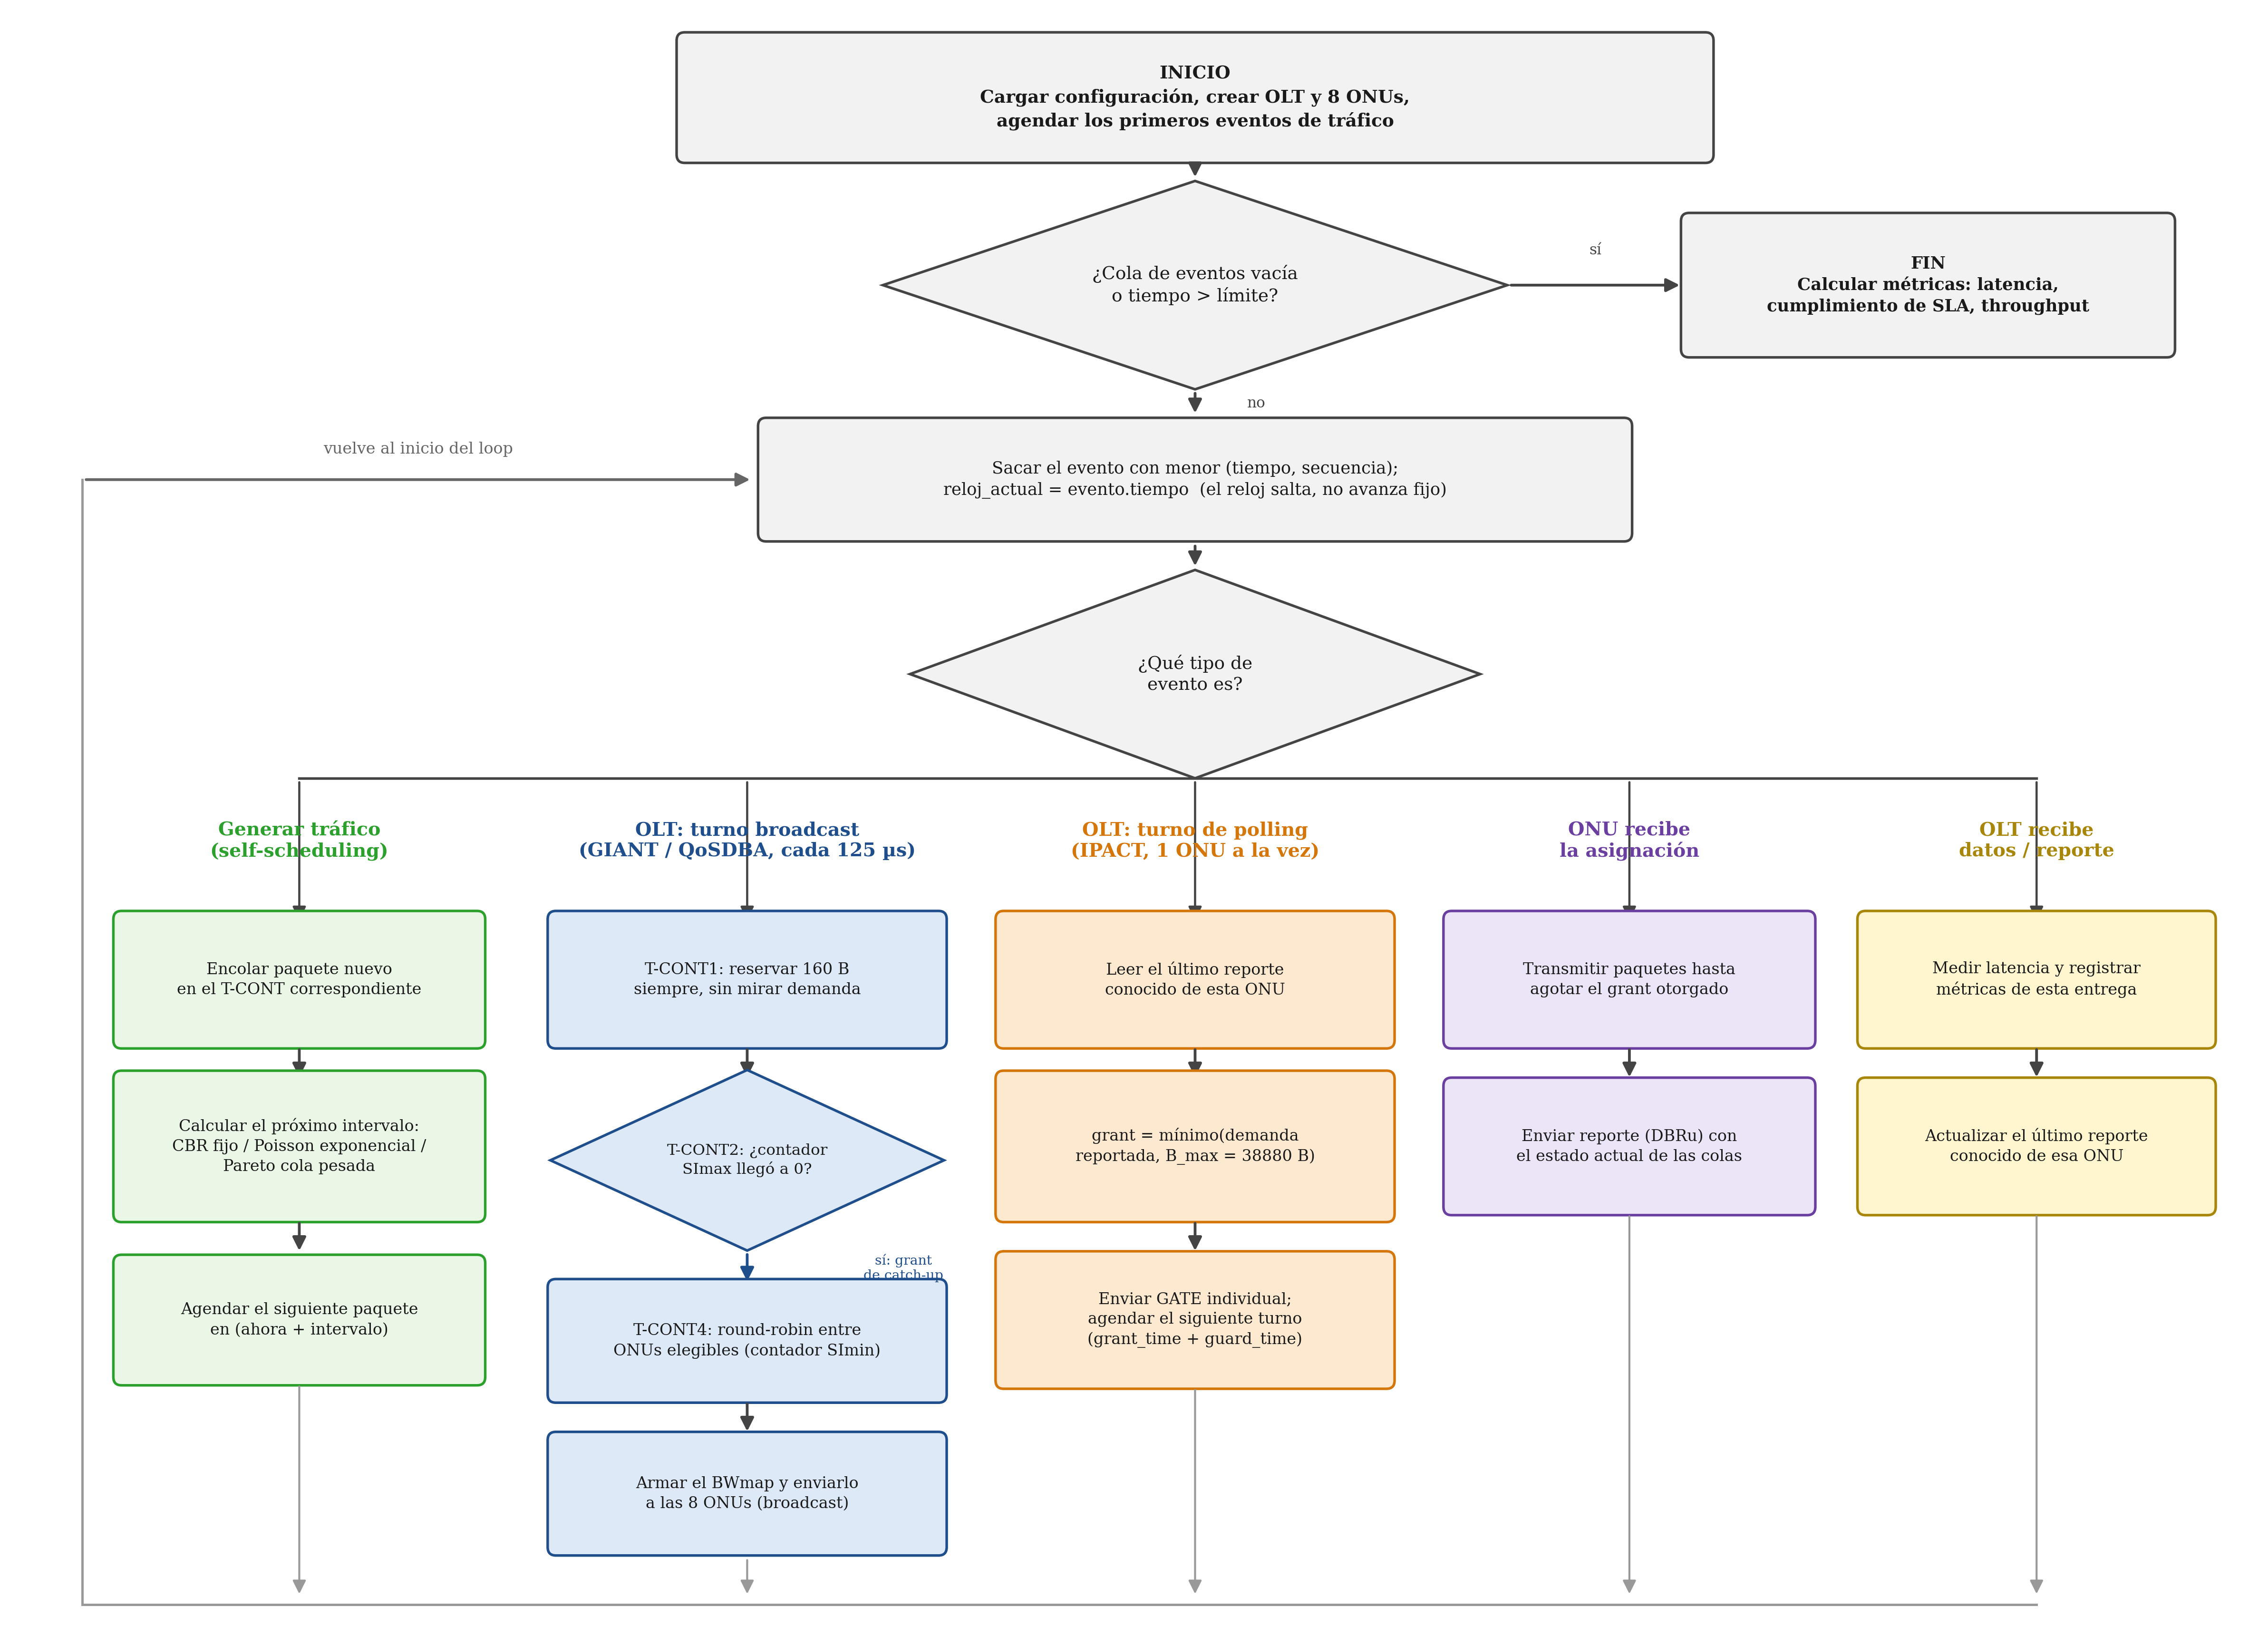
\includegraphics[height=0.8\textheight]{architecture_diagram.png}
    \end{center}
\end{frame}

\begin{frame}[fragile]{El motor de eventos discretos}
    No hay un reloj que avanza de a poco. Hay una lista de eventos
    futuros, ordenada por tiempo, y el simulador salta directo al
    siguiente.

    \begin{lstlisting}[style=pseudo]
mientras la cola de eventos no este vacia:
    evento = sacar el evento mas proximo en el tiempo
    si evento.tiempo > tiempo_limite:
        terminar
    reloj_actual = evento.tiempo   # el reloj salta, no avanza fijo
    handler = handlers[evento.tipo]
    handler(evento)                # puede agendar nuevos eventos
    \end{lstlisting}
\end{frame}

\begin{frame}[fragile]{Generación de tráfico: self-scheduling}
    Cada paquete que se genera agenda su propio sucesor. No existe un
    proceso aparte que esté generando tráfico todo el tiempo.

    \begin{lstlisting}[style=pseudo]
funcion generar_paquete(onu, tcont):
    encolar nuevo paquete en el buffer de tcont
    intervalo = tcont.distribucion.siguiente_intervalo()
    agendar(ahora + intervalo, generar_paquete, onu, tcont)
    \end{lstlisting}

    \footnotesize
    \begin{itemize}
        \item CBR (T-CONT1): intervalo siempre igual
        \item Poisson (T-CONT2): intervalo aleatorio, sin memoria del anterior
        \item Pareto (T-CONT4): intervalo de cola pesada, genera rachas de paquetes
    \end{itemize}
\end{frame}

\begin{frame}{Cómo se ve el tráfico simulado}
    \begin{center}
        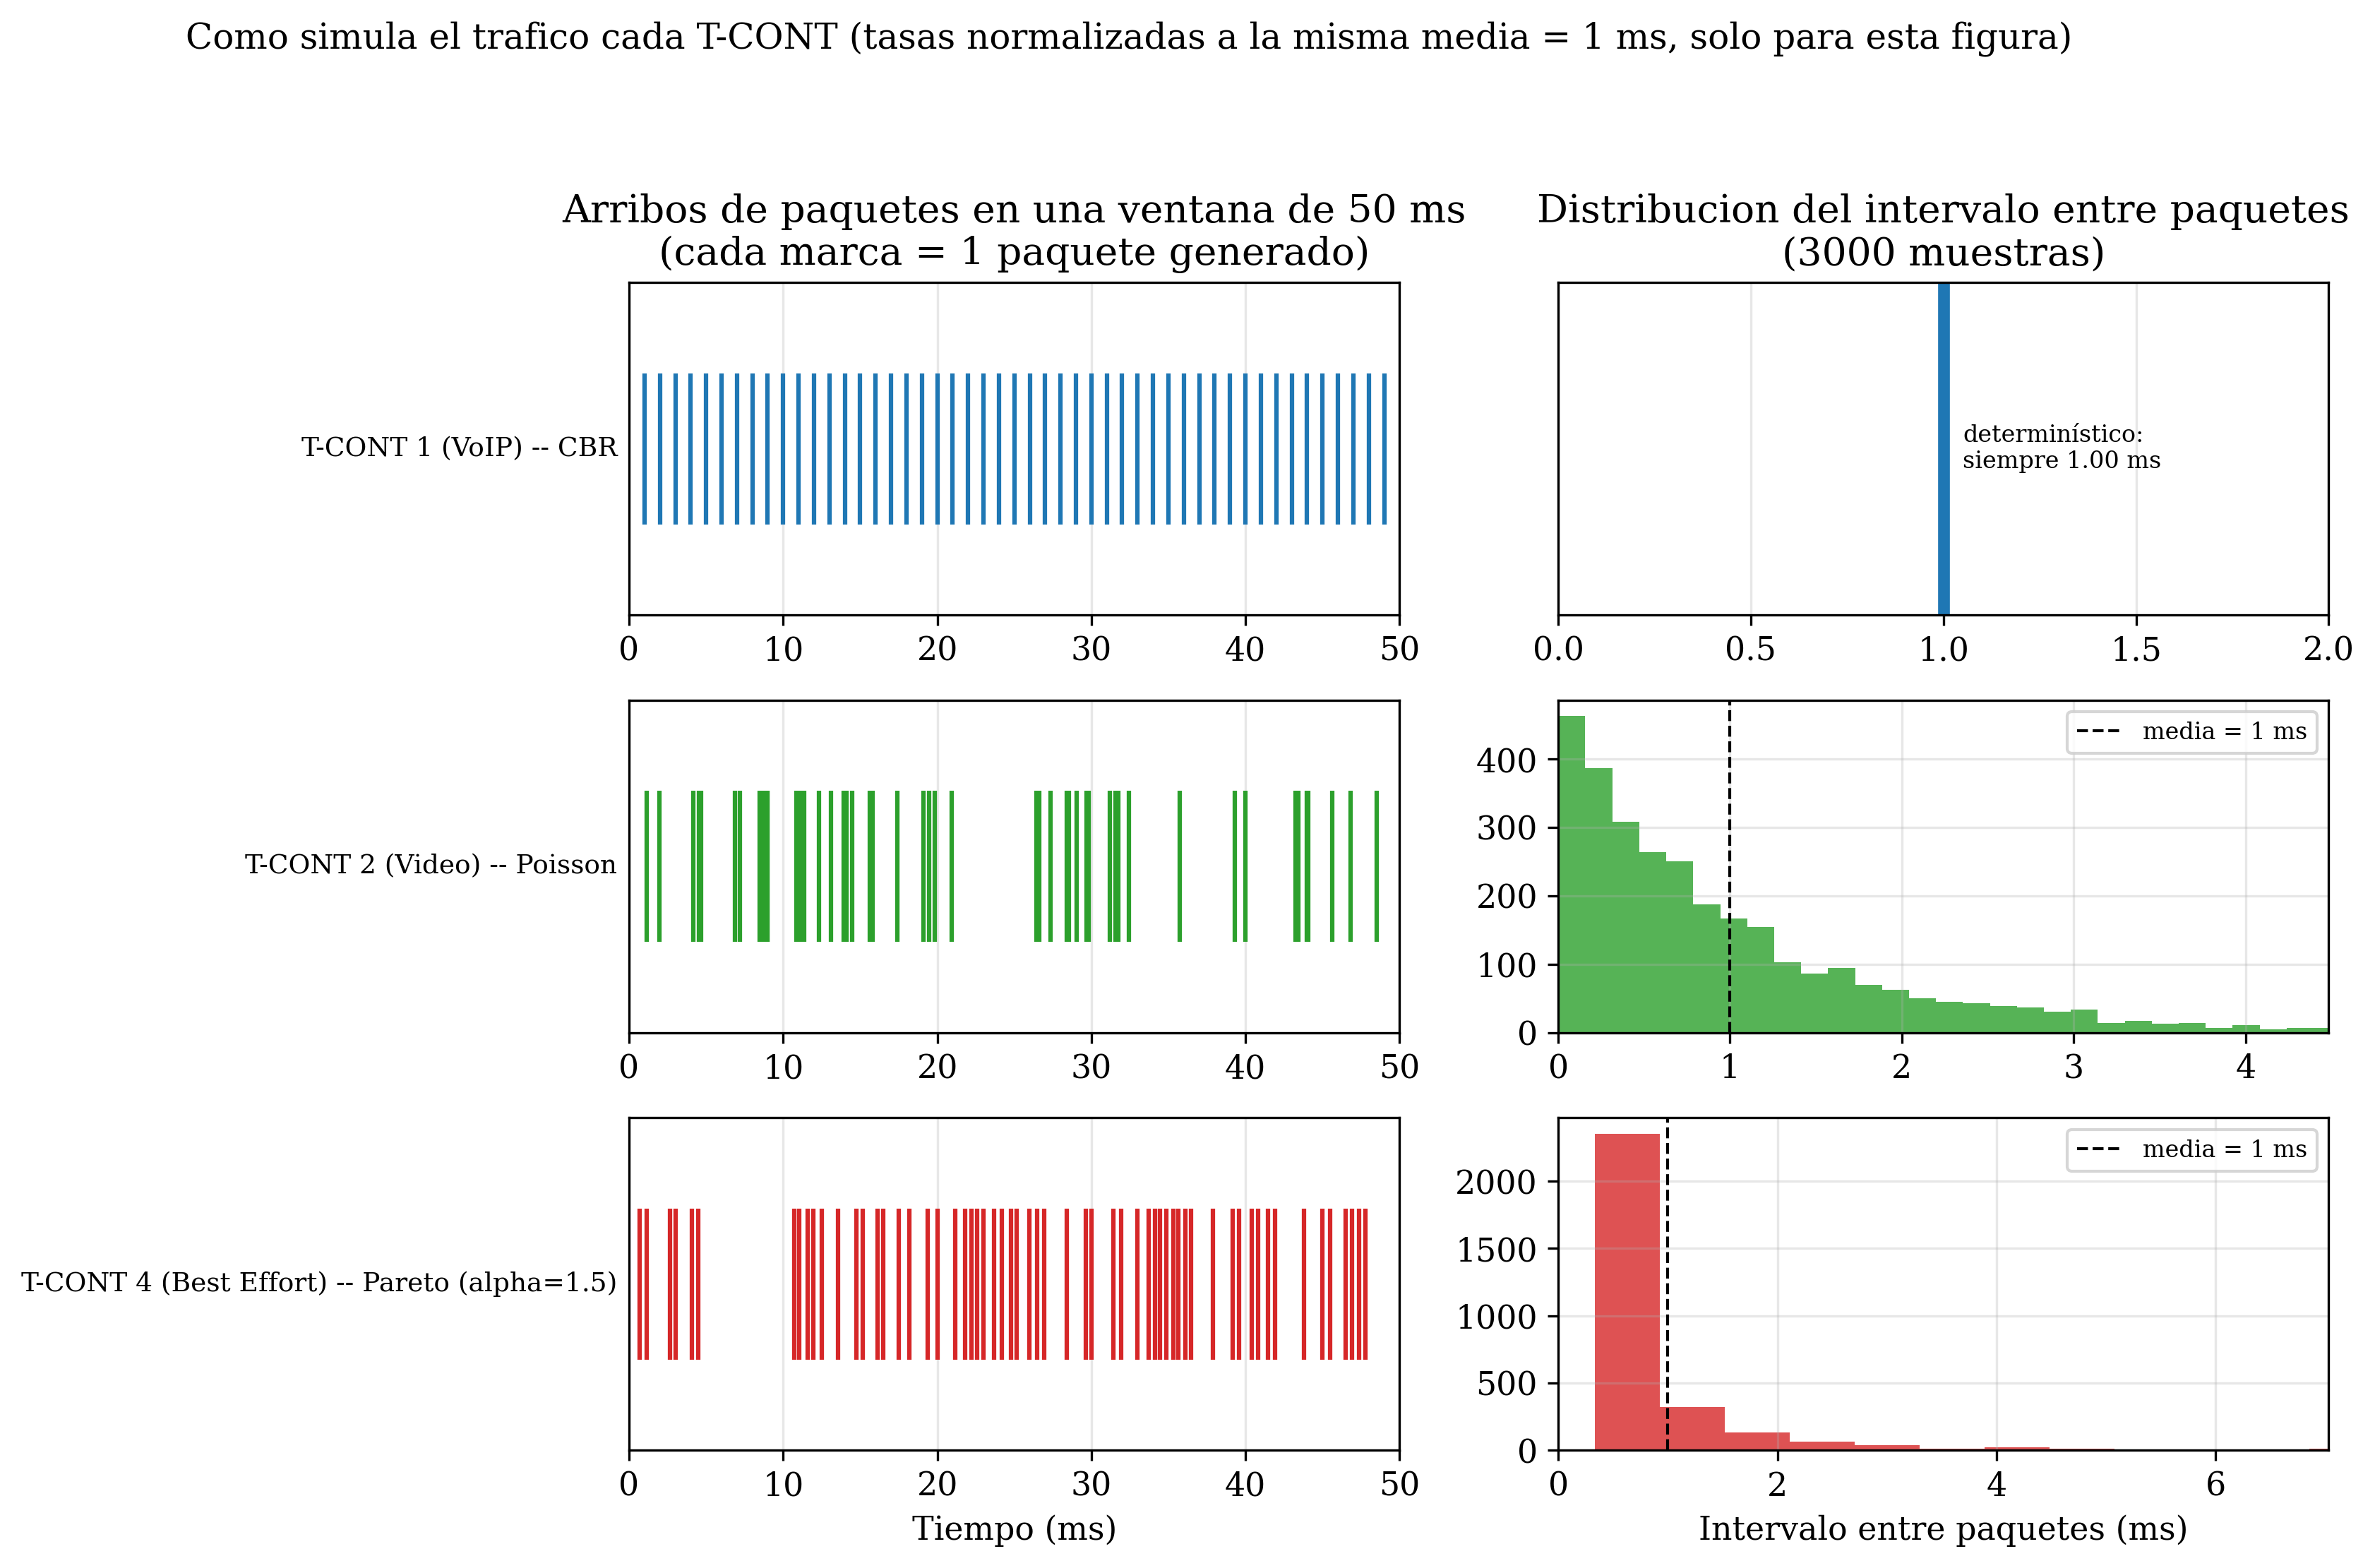
\includegraphics[width=0.55\linewidth]{traffic_generation.png}
    \end{center}
    \footnotesize
    Izquierda: línea de tiempo de arribos (cada marca es un paquete).
    Derecha: histograma del intervalo entre paquetes. Las 3 tasas se
    normalizaron a la misma media solo para esta figura, para comparar la
    forma de cada distribución y no la velocidad.
\end{frame}

\section{Experimentos}

\begin{frame}{Entradas del simulador: de dónde vienen}
    \footnotesize
    \begin{itemize}
        \item \textbf{Parámetros físicos} (tasa, trama, bytes/trama,
              delay) $\rightarrow$ \textbf{ITU-T G.987.1/2/3}, sin
              inventar valores
        \item \textbf{Tasas de tráfico T-CONT1/T-CONT2} $\rightarrow$
              heredadas de Fase 2, T-CONT2 escalado $\times 8$ para
              mantener el mismo \% de capacidad (12.86\%) que con 32 ONUs
        \item \textbf{Cargas de T-CONT4} (200/400/800 Mbps por ONU)
              $\rightarrow$ barrido propio del equipo, mismas razones de
              sobrecarga (64\%/129\%/257\%) que en Fase 2
        \item \textbf{Tabla de SLA} $\rightarrow$ T-CONT1 $\leq$ 2 ms es
              pedido explícito de la profesora; T-CONT2/T-CONT4 son metas
              razonables propuestas por el equipo, no normas del estándar
        \item \textbf{Contadores de GIANT} (SImax=8, SImin=32 tramas)
              $\rightarrow$ interpretación propia de la semántica de
              service-interval de G.987.3, el estándar no fija un valor único
    \end{itemize}
\end{frame}

\begin{frame}{Diseño experimental}
    \begin{itemize}
        \item 3 algoritmos (IPACT, GIANT, QoSDBA) $\times$ 3 cargas de
              T-CONT4 (200, 400 y 800 Mbps por ONU, entre 64\% y 257\% de
              la capacidad disponible)
        \item 10 repeticiones por escenario, 10 segundos simulados cada
              una (con 1 segundo de calentamiento que no se mide)
        \item Se mide latencia, throughput, pérdida y cumplimiento de SLA
              por cada ONU y cada T-CONT
    \end{itemize}
\end{frame}

\section{Resultados}

\begin{frame}{Validación: cotas teóricas vs. simulación}
    \footnotesize
    No es una cola M/M/1 clásica (los grants son deterministas o por
    contador), pero sí hay 2 cotas cerradas que se pueden derivar y
    contrastar directamente:

    \vspace{0.2cm}
    \textbf{(a) Ciclo de polling IPACT:}
    $[N \cdot t_{guard},\; N \cdot (B_{max} \cdot 8/R + t_{guard})]
    = [8\,\mu s,\; 1008\,\mu s]$.
    Medido: máximo exactamente \textbf{1008.000 $\mu$s} bajo saturación
    (400/800 Mbps/ONU) — calza exacto con la cota teórica.

    \vspace{0.2cm}
    \textbf{(b) Latencia de T-CONT1 en GIANT/QoSDBA} (grant fijo
    incondicional + CBR): $L_{max} = T_{trama} + T_{prop} + T_{tx}
    = 125 + 100 + 1.03 = \textbf{226.03}\,\mu s$.
    Medido: \textbf{226.0288 $\mu$s}, con \textbf{IC95\%=0} (sin
    aleatoriedad en ese camino) — confirma que la cota es exacta, no una
    aproximación.
\end{frame}

\begin{frame}{Resultado central: cumplimiento del SLA}
    \begin{center}
        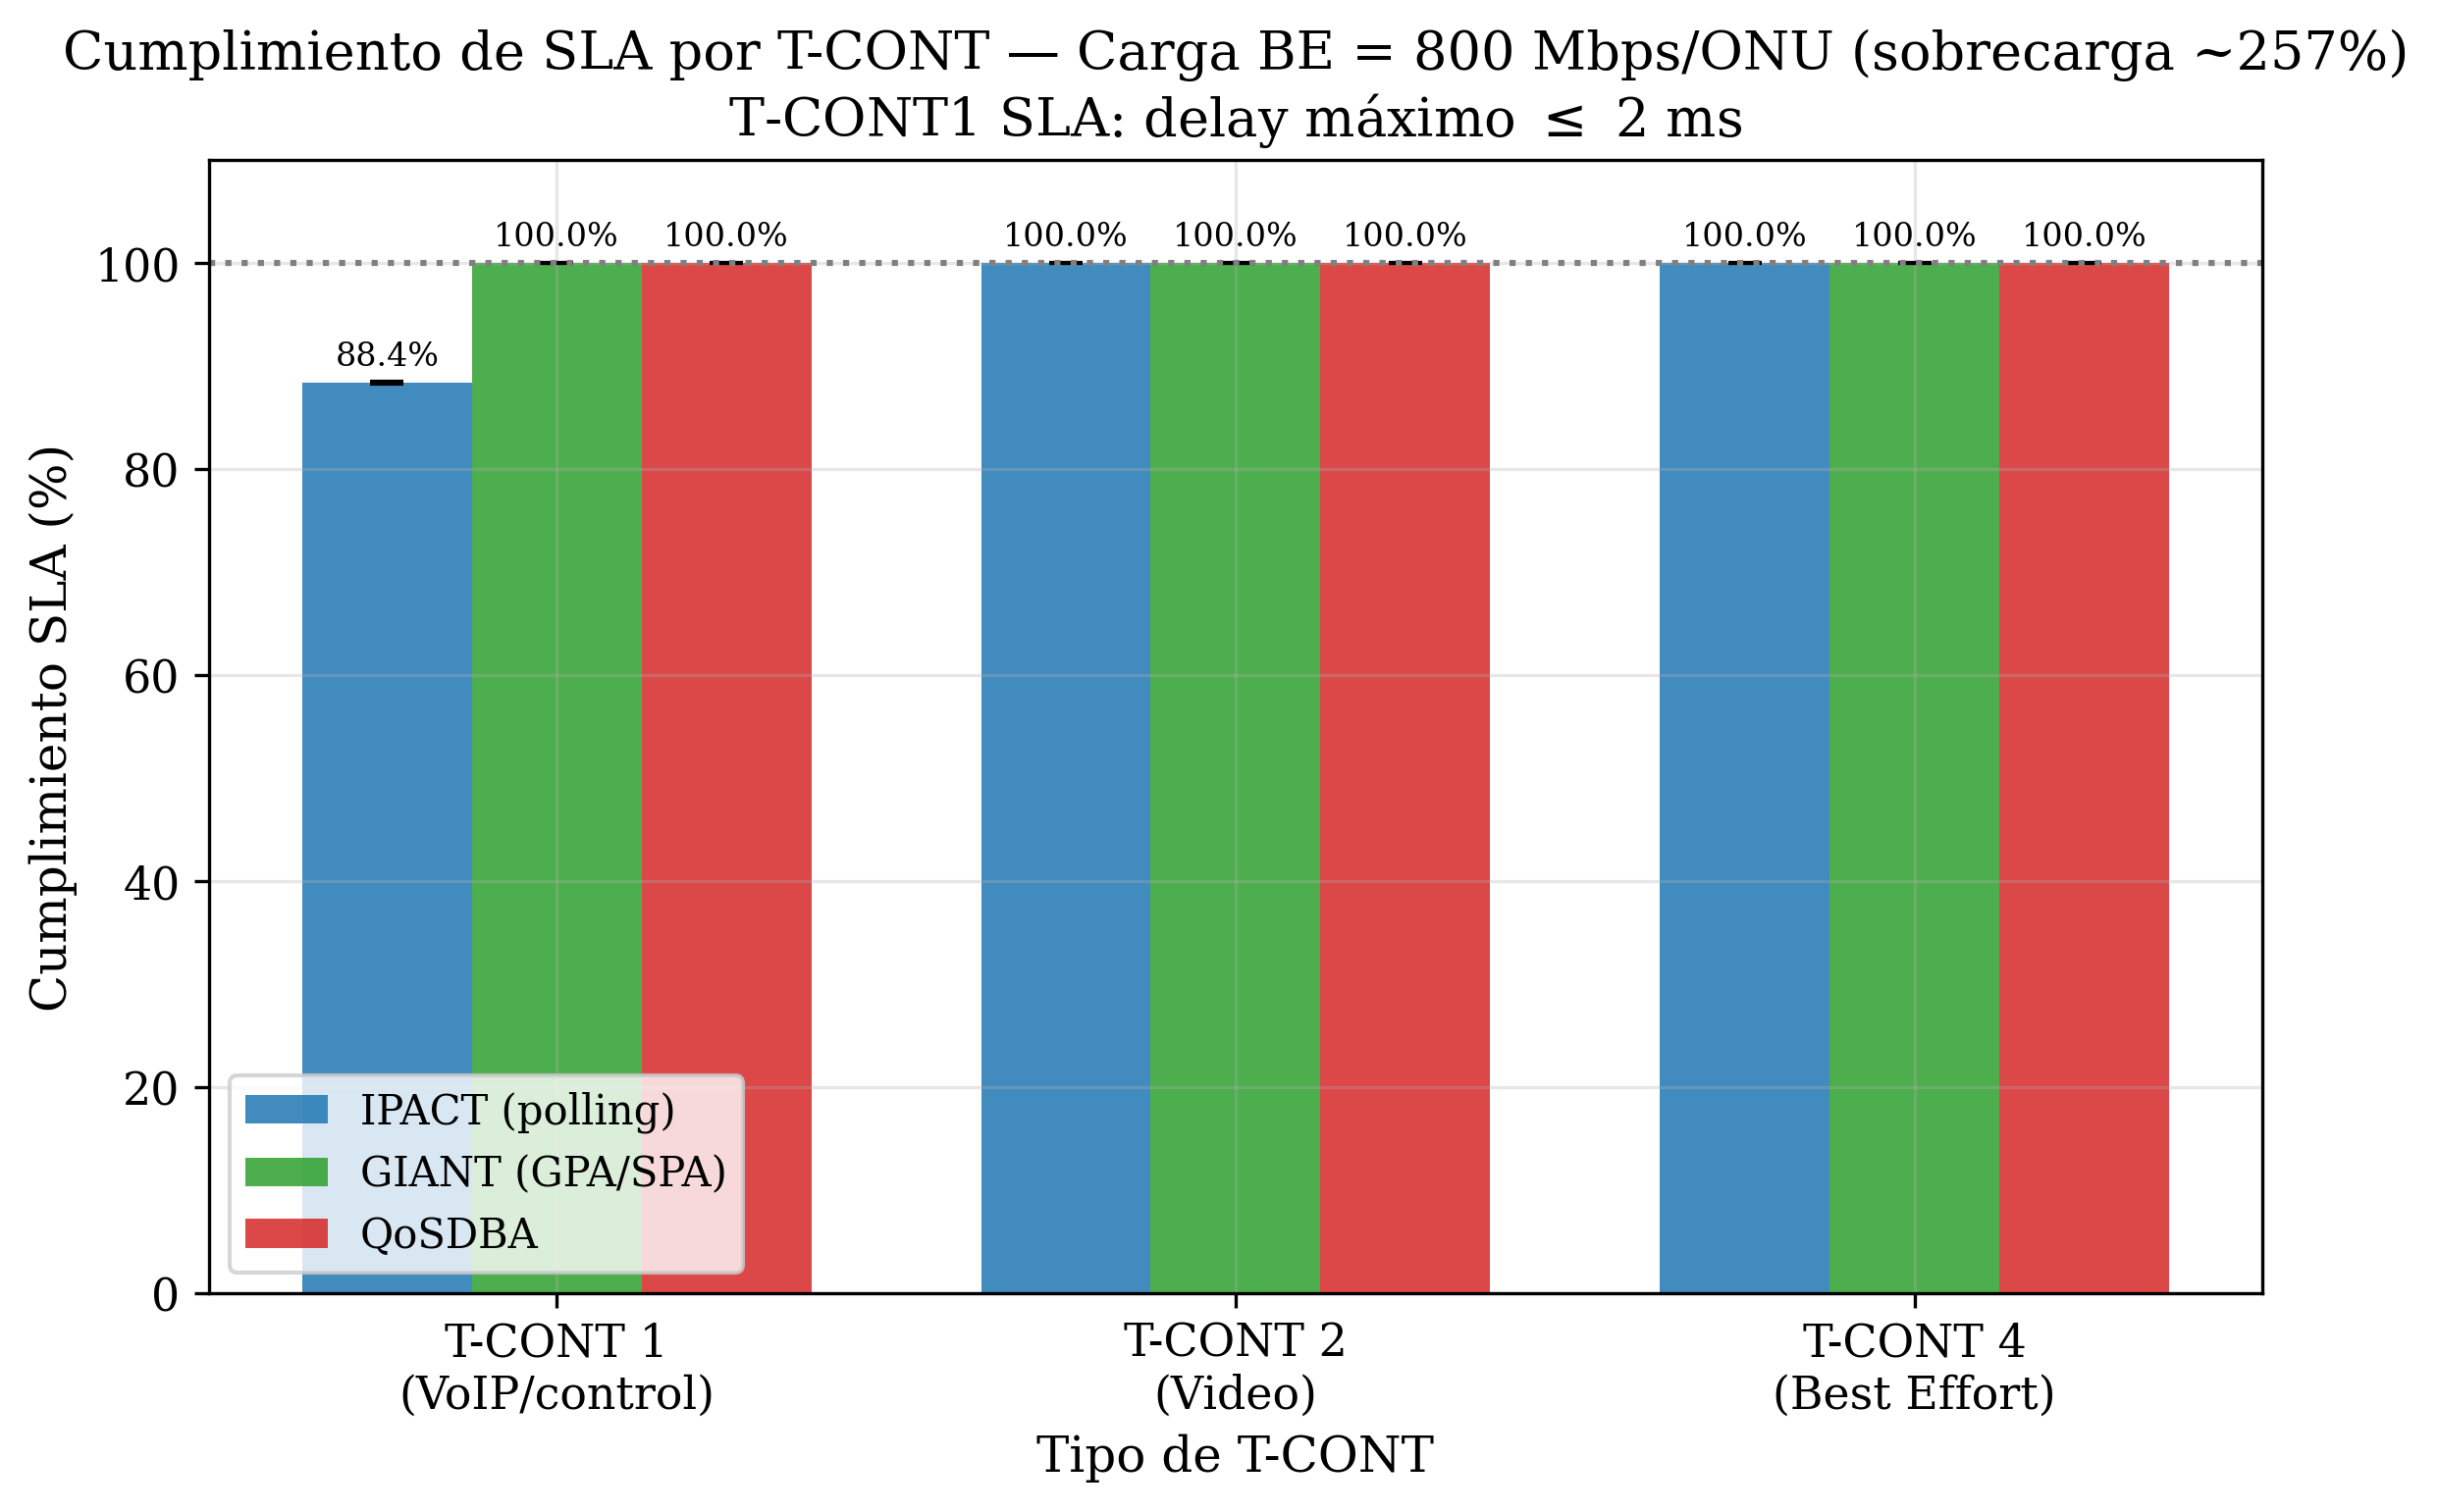
\includegraphics[width=0.6\linewidth]{sla_compliance_by_tcont.png}
    \end{center}
    \footnotesize
    A 800 Mbps por ONU, IPACT cae a \textcolor{rojoDBA}{\textbf{88.4\%}}
    en T-CONT1 (voz). GIANT y QoSDBA se quedan en 100\% en los 3 T-CONTs.
\end{frame}

\begin{frame}{Por qué falla IPACT}
    \begin{center}
        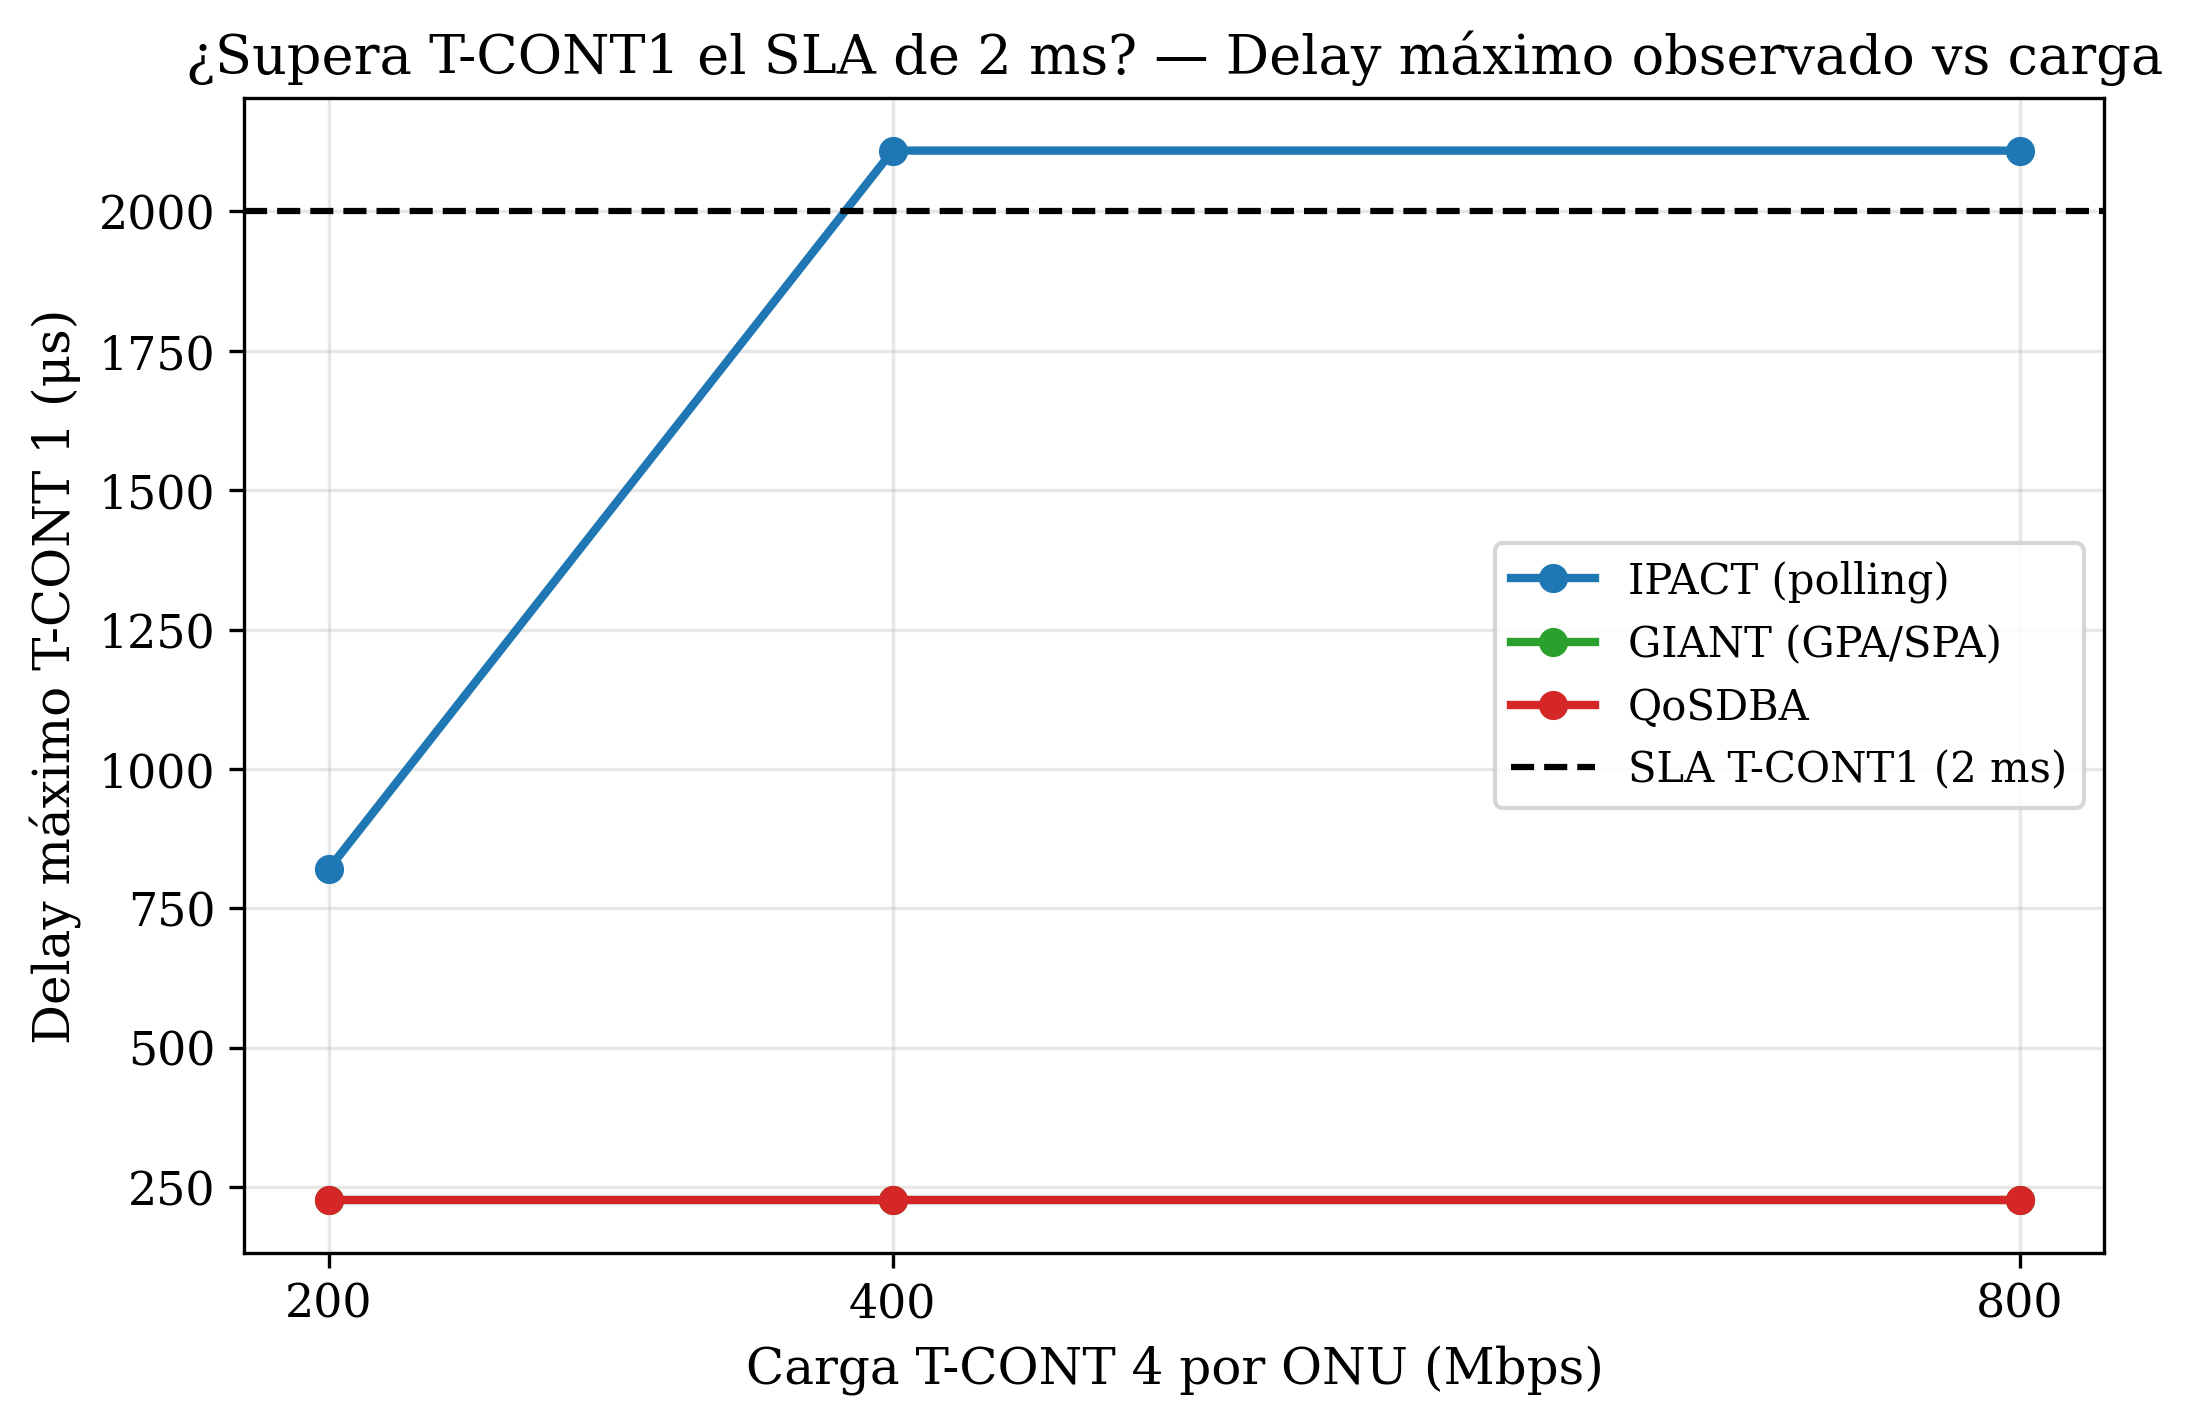
\includegraphics[width=0.58\linewidth]{max_delay_tcont1_vs_load.png}
    \end{center}
    \footnotesize
    A partir de 400 Mbps por ONU, el delay máximo de IPACT cruza la línea
    de SLA (2 ms). GIANT y QoSDBA se quedan planos en
    \textbf{226 $\mu$s}, sin importar la carga.
\end{frame}

\begin{frame}{El mecanismo detrás}
    \begin{center}
        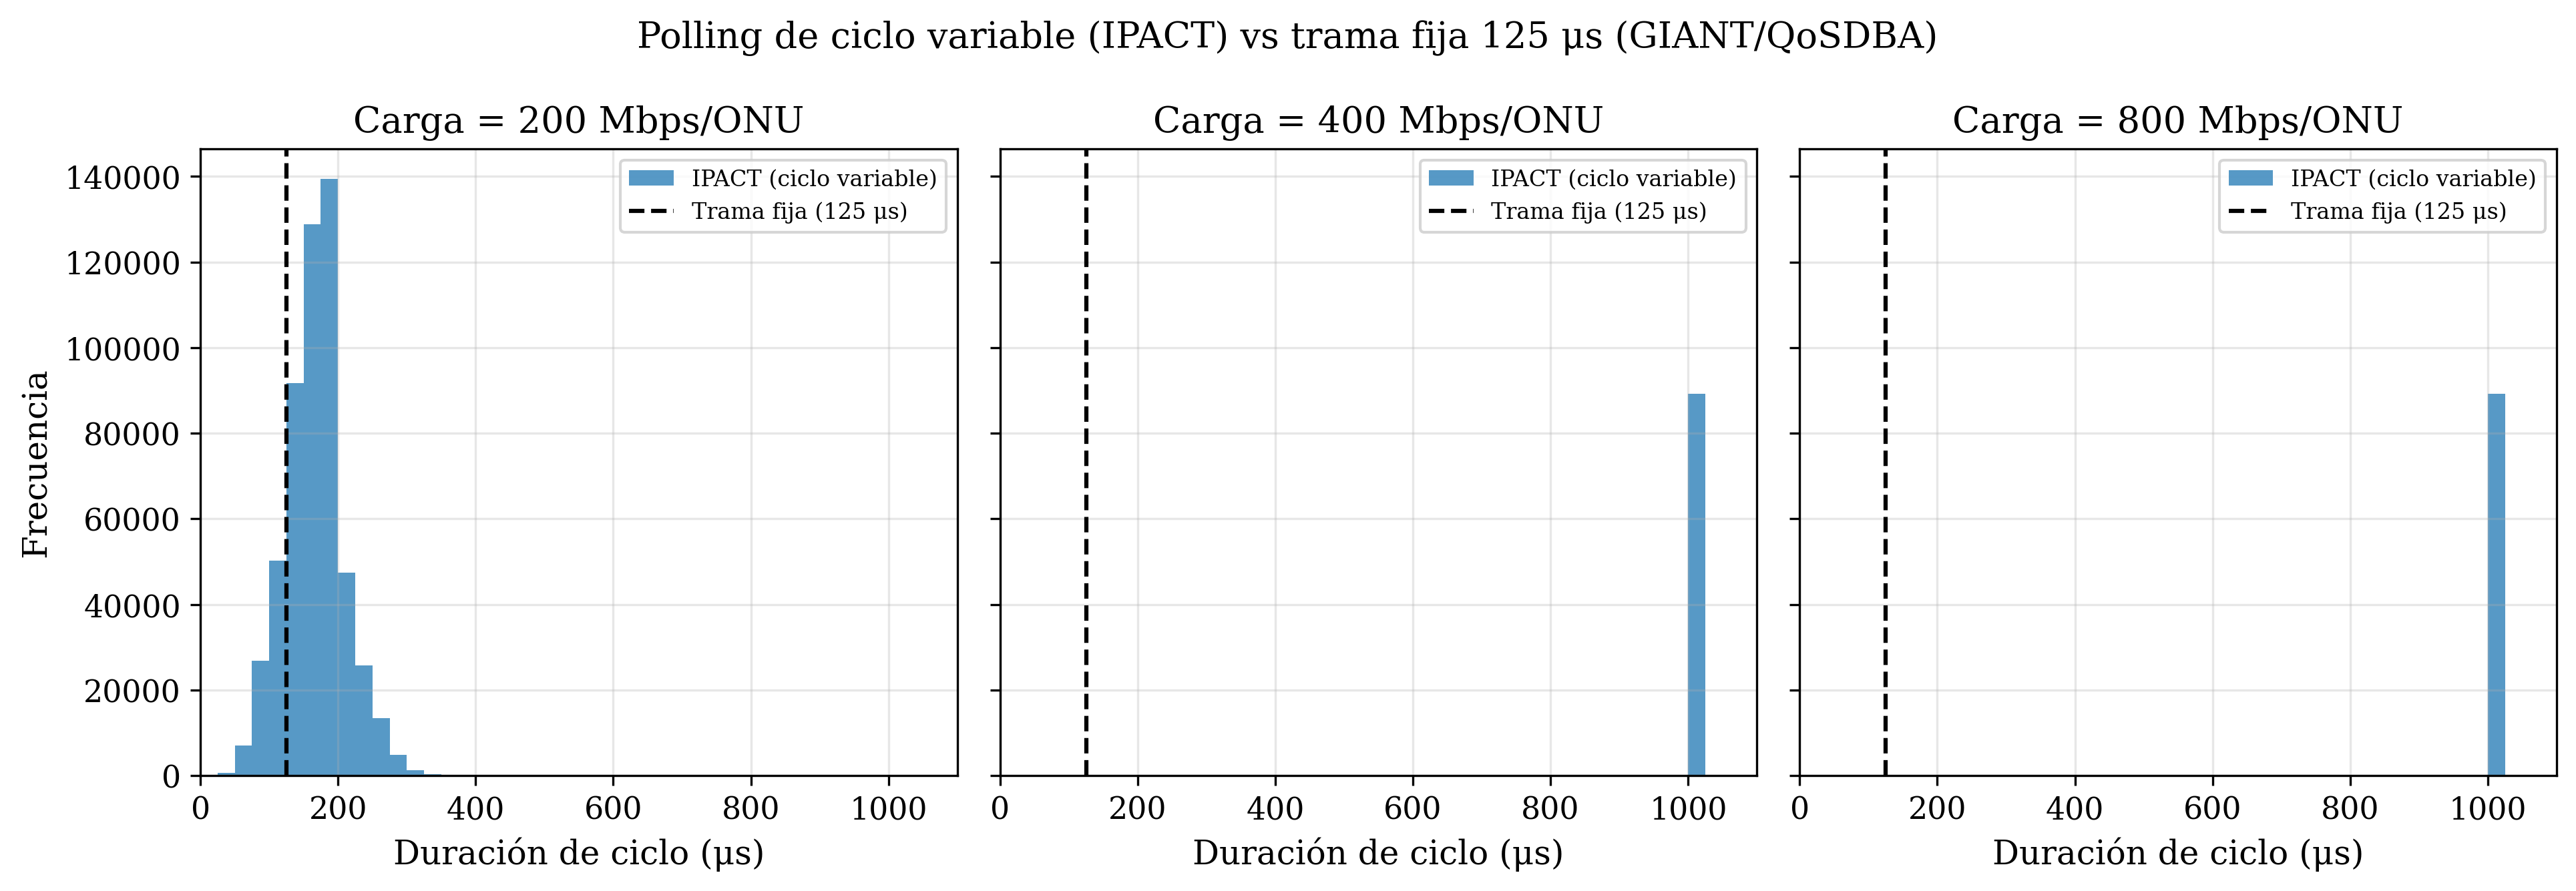
\includegraphics[width=\textwidth]{cycle_time_distribution.png}
    \end{center}
    \footnotesize
    Bajo carga alta, el ciclo de IPACT se vuelve constante en
    \textbf{1008 $\mu$s} (el máximo teórico para 8 ONUs). GIANT y QoSDBA
    usan siempre la trama fija de 125 $\mu$s.
\end{frame}

\begin{frame}{Confiabilidad estadística}
    \footnotesize
    \begin{itemize}
        \item \textbf{10 réplicas i.i.d.} por escenario (semillas
              6767-6776), 1 s de \textit{warmup} descartado de 10 s
              simulados, siguiendo Law \& Kelton (2000)
        \item IC95\% calculado como $\bar{y} \pm 1.96 \cdot s/\sqrt{10}$
              sobre las 10 réplicas, reportado para cada métrica en
              \texttt{results.csv}
        \item \textbf{Ejemplo de error relativo} (IC95 / media)
              en T-CONT1, IPACT a 400 Mbps/ONU: latencia media
              $1613.08 \pm 0.33\,\mu s$ $\rightarrow$ error relativo
              $\approx 0.02\%$ — variabilidad entre réplicas muy baja
        \item Donde el algoritmo es determinista (T-CONT1 bajo
              GIANT/QoSDBA), el IC95\% es exactamente \textbf{0}: no hay
              fuente de aleatoriedad en ese camino, las 10 réplicas son
              idénticas
    \end{itemize}
\end{frame}

\section{Conclusiones}

\begin{frame}{Conclusiones}
    \begin{itemize}
        \item Cumplir el SLA de voz no es automático, depende de cómo
              decide el algoritmo de DBA
        \item Reservar ancho de banda sin condiciones (GIANT, QoSDBA)
              garantiza el SLA de voz en cualquier escenario que probamos
        \item Asignar según un reporte de demanda puede fallar justo
              cuando más se necesita: bajo carga alta y con un reporte
              desactualizado
        \item Esto tiene un costo: QoSDBA es más simple pero pierde
              eficiencia en el tráfico de datos (ver apéndice)
    \end{itemize}

    \vspace{0.2cm}
    \footnotesize
    \textbf{Trabajo futuro:} ranging dinámico (ONUs a distancias
    distintas, RTT variable en vez de fijo), GIANT operando a nivel
    T-CONT en vez de 1:1 con la ONU, más de un T-CONT del mismo tipo por
    ONU, y ONUs heterogéneas (distintos perfiles de tráfico simultáneos).
\end{frame}

\begin{frame}
    \vfill
    \centering
    \Large Gracias\\
    \vspace{0.3cm}
    \large ¿Preguntas?
    \vfill
\end{frame}

\appendix
\section*{Apéndice}

\begin{frame}{Apéndice: dashboard resumen}
    \begin{center}
        
\includegraphics[height=0.78\textheight]{summary_dashboard.png}
    \end{center}
\end{frame}

\begin{frame}{Apéndice: eficiencia agregada}
    \begin{center}
        
\includegraphics[width=0.56\linewidth]{throughput_vs_load.png}
    \end{center}
    \footnotesize
    A 800 Mbps por ONU, IPACT y GIANT entregan entre 94\% y 97\% de la
    capacidad disponible. QoSDBA se queda en 73\%: su reparto
    proporcional del tráfico de datos deja capacidad sin usar.
\end{frame}

\end{document}
